The Lam{\'{e}} constants defined for Hooke's fourth-order elastic material tensor (\ref{eq:hook}) can be expressed by the Young's modulus $E$, the Poisson's ratio $\nu$ and the shear modulus $G$ (so-called {\sl enginering constants}) which can be obtained experimentally.
\begin{eqnarray}
\mu     & = & \ttfrac{E}{2(1+\nu)}\,=\,G \\[1.5ex]
\lambda & = & \ttfrac{E\nu}{(1+\nu)(1-2\nu)}\,=\,\ttfrac{2G\nu}{(1-2\nu)}
\end{eqnarray}

In many technical applications considering small strains, the elastic material parameters are assumed to be constant, and the stress-strain curves are nearly linear. However, the typical response of certain geological materials to monotonic loading (without load reversal) shows a nonlinear stress-strain behavior. Considering only elastic effects during load application, Hooke's law cannot be used to describe the observed material properties. Therefore, so-called pseudo-elastic constitutive models are frequently used for the analysis of nonlinear stress-strain curves, particularly in soil and rock mechanics. In a generalized manner, they are based on the assumption of an explicit stress-strain relation considering a stress- and strain-dependent material matrix:
\begin{equation}
\mio{\sigma}{}{}\,=\,\fourtens{\mathcal{C}}(\mio{\sigma}{}{},\mio{\varepsilon}{}{})\ccdot\mio{\varepsilon}{\mathrm{e}}{}\,.
\label{elasticity_nonlin}
\end{equation}

Based on the so-called {\sl Lubby1} model (cf. \cite{Lux:1984}), a nonlinear elastic approach with strain-dependent Young's modulus
\begin{equation}
E(\varepsilon_{\mathrm{v}})\,=\,\frac{E_0}{1+a\,\varepsilon_{\mathrm{v}}^n}
\label{lubby1_ev}
\end{equation}
but constant Poisson's ratio is proposed. Here, $\varepsilon_{\mathrm{v}}$ is the equivalent strain, and $E_0$, $a$ as well as $n$ are material parameters . The equivalent strain is defined by
\begin{equation}
\varepsilon_{\mathrm{v}}\,=\,
\sqrt{\frac{2}{3}\,\mio{\varepsilon}{\mathrm{e}}{}\ccdot\mio{\varepsilon}{\mathrm{e}}{}}\,.
\end{equation}

\subsubsection*{Problem definition}

Triaxial short-term compression under axisymmetric conditions is carried out to verify the nonlinear elastic isotropic material model (modified Lubby1 approach). For the calculation, the cross-section of a cylindrical sample with a radius of 30~mm and a height of 120~mm is studied. The loading in principal axes includes a radial pressure as well as an axial displacement, and is realized in two steps. It is resulting in a homogeneous stress-strain state. Details of the model (geometry, mesh, boundary conditions) according to K.-H. Lux and F. Werunsky (unpublished report, 2008) are presented in Fig.~\ref{triax_model_lubby1}.

\begin{figure}[!htb]
\begin{center}
\includegraphics[width=0.2\textwidth]{M/figure/svv_model.eps}
\hspace*{10.0ex}
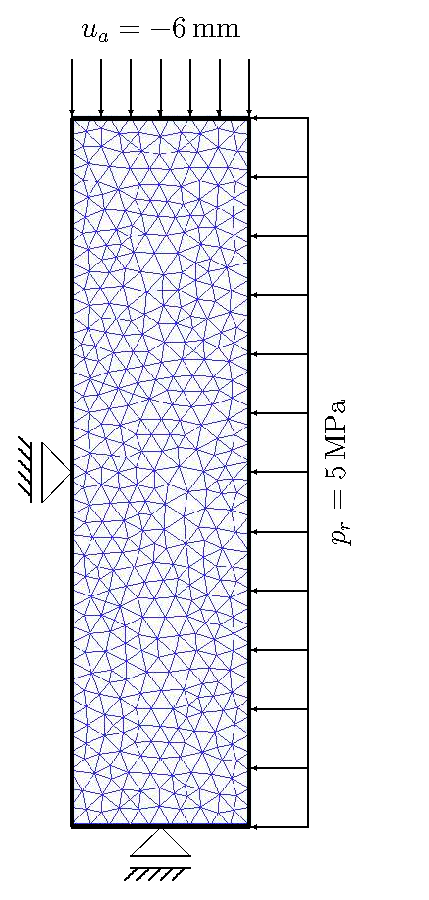
\includegraphics[width=0.25\textwidth]{M/figure/svv_mesh.eps}
\end{center}
\caption{Triaxial compression of a cylindrical sample. Axisymmetric model. Left: Geometry. Right: Finite element grid and boundary conditions.} 
\label{triax_model_lubby1}
\end{figure}

\begin{figure}[!htb]
\begin{center}
\includegraphics[width=0.6\textwidth]{M/figure/svv_loadhistory.eps}
\end{center}
\caption{Triaxial compression of a cylindrical sample. Loading history for short-term experiments. Radial casing pressure (stress rate $\dot{p}{}_r=0.25$\,MPa$\cdot$s$^{-1}$) with subsequent axial displacement (strain rate $\dot{\varepsilon}{}_a=3.47\cdot 10^{-5}$\,s$^{-1}$).} 
\label{triax_loadhist_lubby1}
\end{figure}

\subsubsection*{Initial and boundary conditions}

Initial conditions do not have to be given for the problem under consideration. As the bottom edge is fixed in vertical direction, the left-hand edge is fixed in horizontal direction for symmetry reasons (axis of rotation). On the right-hand edge initially a radial casing pressure of 5~MPa is applied within 20~seconds with a constant stress rate. While keeping constant this radial pressure, a subsequent stroke-driven axial compressive loading is applied within the following 1\,440~seconds with a constant strain rate. The maximum axial displacement is 6~mm which corresponds to a 5\% reduction of the sample's height (for the complex loading history cf. Fig.~\ref{triax_loadhist_lubby1}).

\subsubsection*{Material properties}
 
The material parameters referring to the modified Lubby1 relation~(\ref{lubby1_ev}) are summarized in Tab.~\ref{matpar_lubby1}. Within this context, the initial Young's modulus and the Poisson's ratio are close to values known for rock salt.
 
\vskip 3.0ex
 
\begin{table}[!htb]
\centering
\begin{tabular}{lll}
\hline\hline\noalign{\smallskip}
Property & Value & Unit \\
\noalign{\smallskip}\hline\noalign{\smallskip}
Poisson's ratio $\nu$             & 0.335   & --  \\
initial Young's modulus $E_0$     & 21\,400 & MPa \\
factor $a$ in (\ref{lubby1_ev})   & 2\,750  & --  \\
exponent $n$ in (\ref{lubby1_ev}) & 1.0     & --  \\
\noalign{\smallskip}\hline\hline
\end{tabular}
\caption{Material parameters}
\label{matpar_lubby1}
\end{table}

\subsubsection*{Results}

The representation of the axial stress vs. the axial strain in Fig.~\ref{triax_res_lubby1} shows on exemplarily chosen material parameters the noticeable difference between the linear (Hooke's model) and the nonlinear (modified Lubby1 model) elastic models even at small strains. Within the contect of the studied case, the stress response will be overestimated by a multiple using the linear Hooke's law. 

\clearpage

\begin{figure}[!htb]
\begin{center}
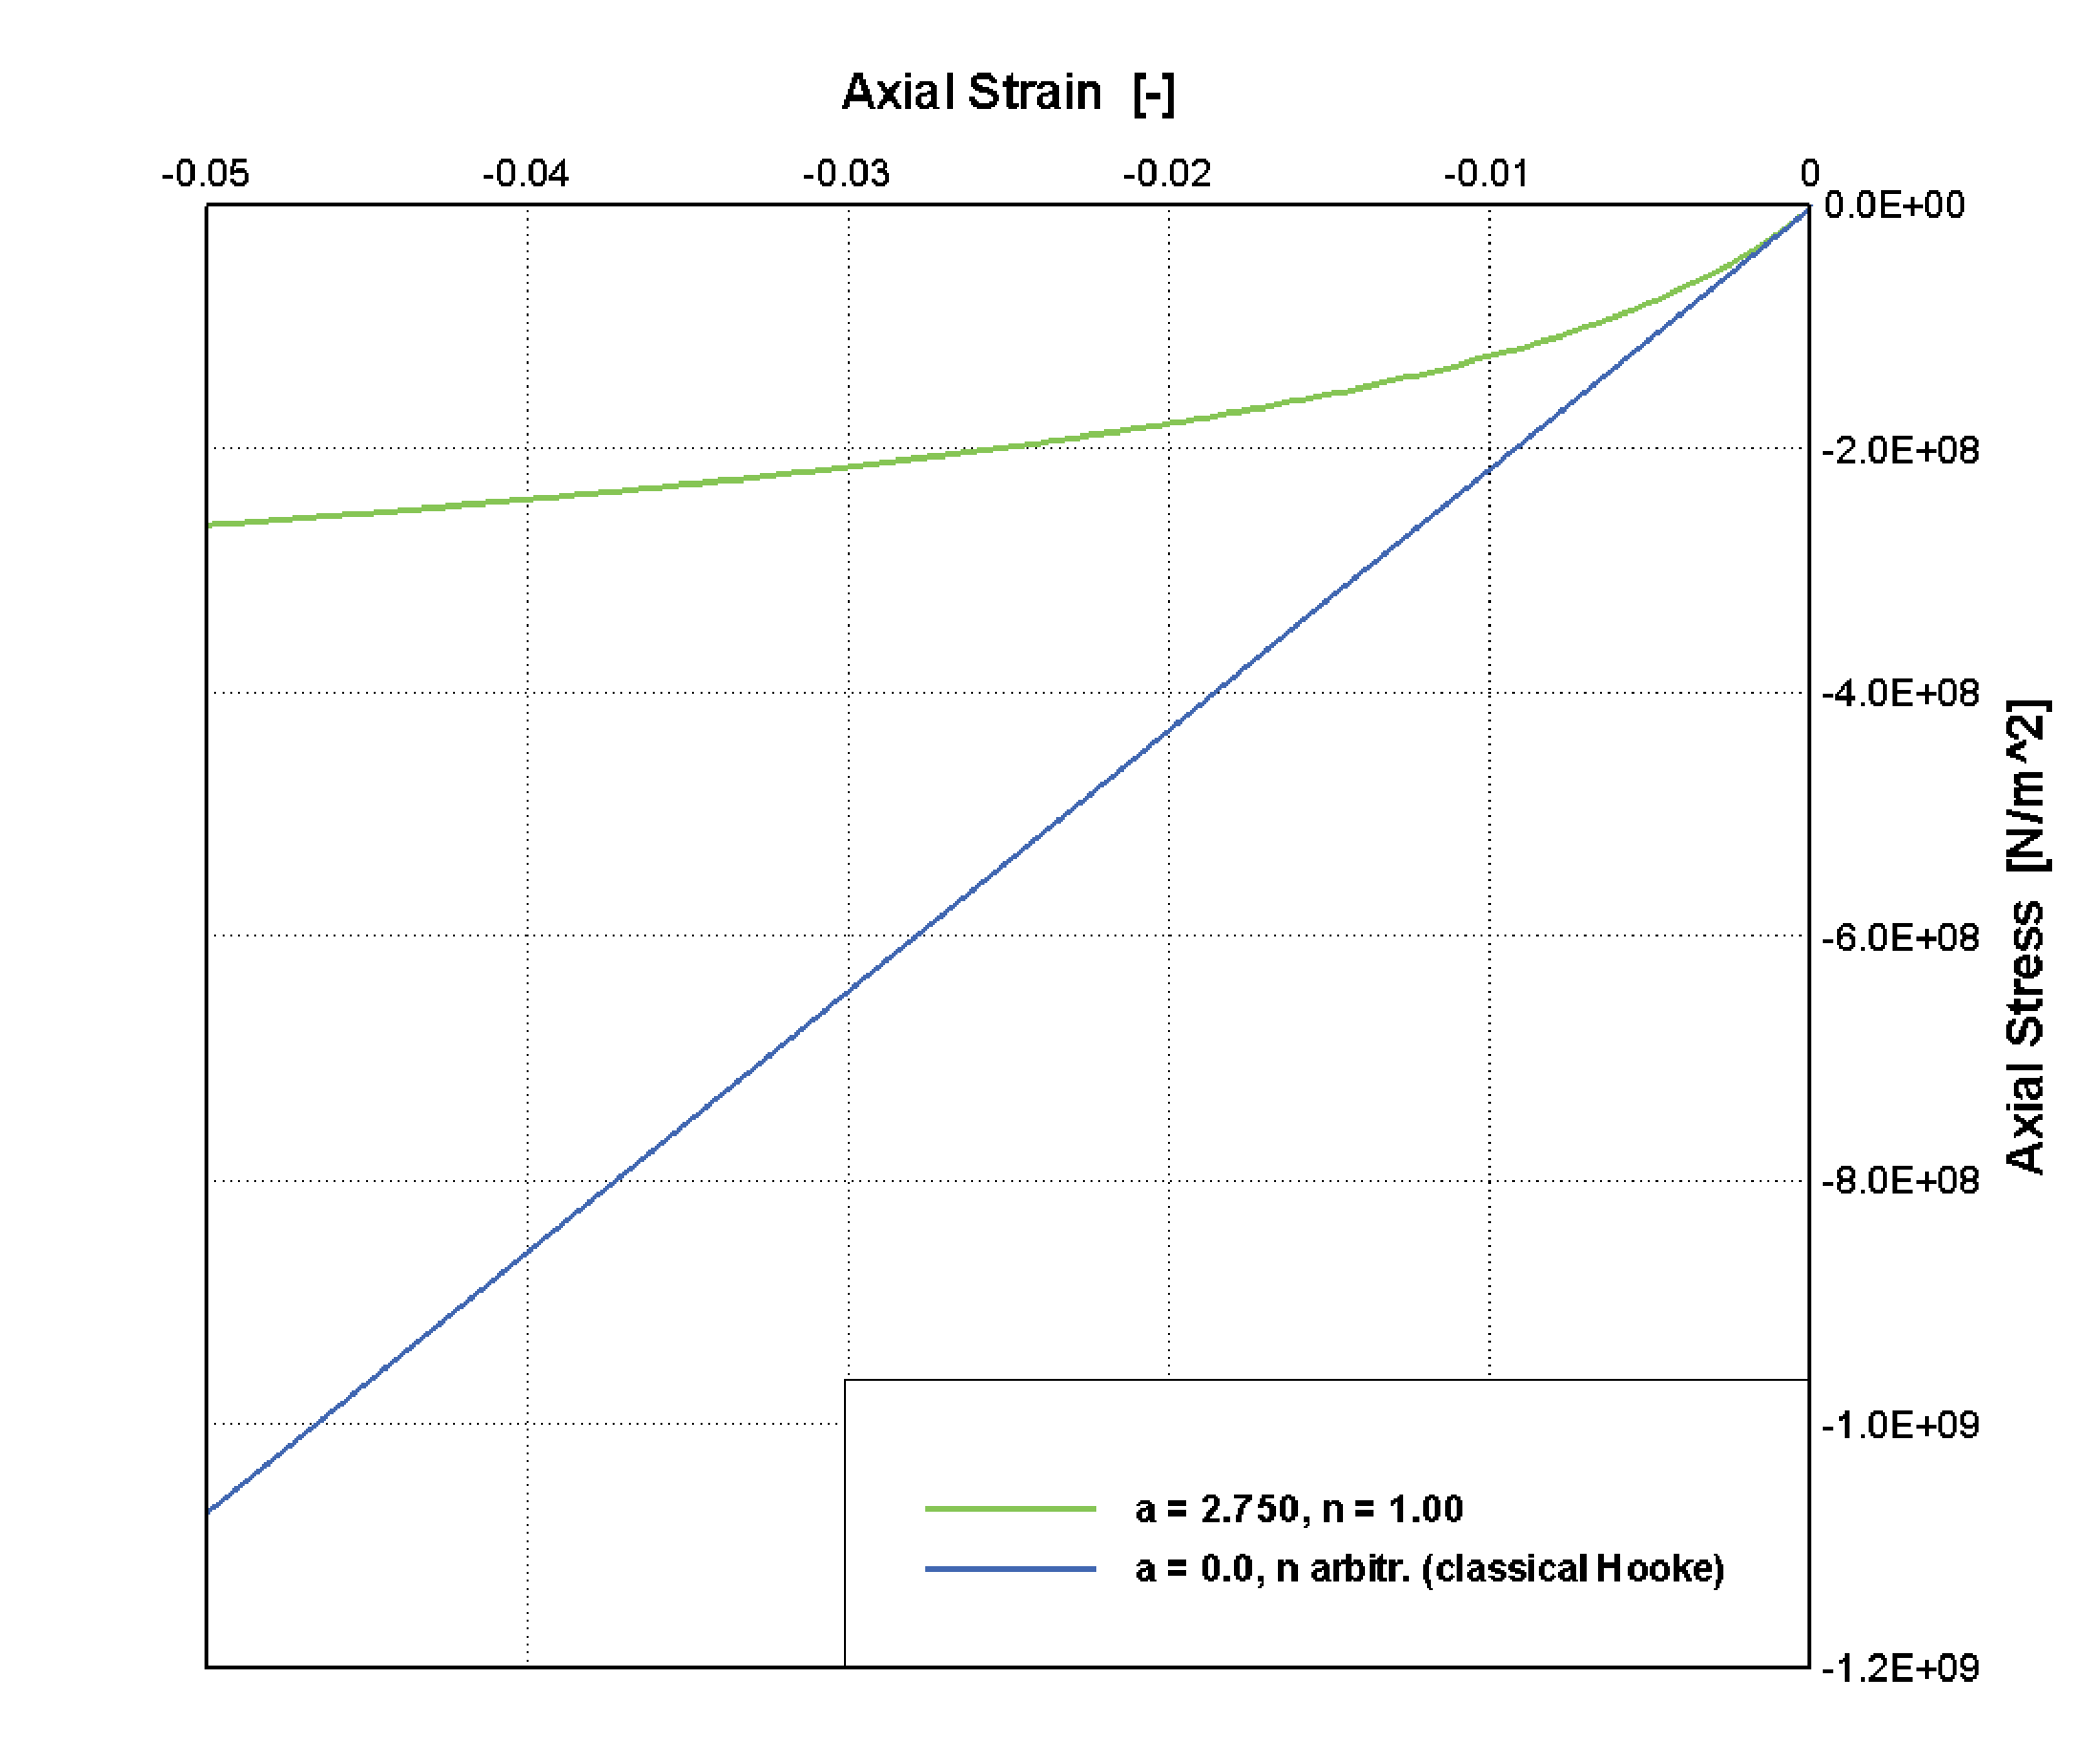
\includegraphics[width=0.6\textwidth]{M/figure/svv_e_stress_strain_hooke_lubby1m.eps}
\end{center}
\caption{Triaxial compression of a cylindrical sample. Stress-strain curves regarding the axial load response. Comparison of linear elastic (Hooke) and nonlinear elastic (modified Lubby1~(\ref{lubby1_ev})) material models.} 
\label{triax_res_lubby1}
\end{figure}

\vskip 4.0ex

\subsubsection*{Benchmark deposit}

\begin{tabular}{|l|l|l|}
  \hline
  Benchmark & Problem type & Path in benchmark deposit \\
  \hline
 \emph{m\_triax\_lubby1} & M & benchmarks\verb \M\ \\
  \hline
\end{tabular}


